Her følger en beskrivelse af kildekode fil strukturen og hvordan denne omsættes til de forskellige enheder.

\subsection{Filstruktur}
På figur \ref{fig:filstruktur1} er filstrukturen vist for software implementeringen.
De er delt op i tre mapper: PC, CSS-hovedenhed og X10-udtag.

\begin{figure}[!htb]
     \centering
     { 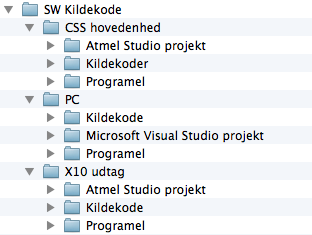
\includegraphics{billeder/Filstruktur1}}
     \caption{Overordnet filstruktur}
     \label{fig:filstruktur1}
\end{figure}

I hver mappe ligger de rå kildekoder, et projekt i det tilhørende udviklingsprojekt og de rå programmer som bruges på hver platform, hhv. .exe og .hex til PC og CSS-hovedenhed og X10-udtag.
I tabel \ref{table:Udviklingsprogrammer} er vist hvilke udviklingsværktøjer der er brugt til de forskellige platforme.

\begin{table}[htb]
	\caption{Udviklingsplatforme til software udviklingen}
	\centering
	\begin{tabular}{|c|c|}
		\hline 
		\textbf{Enhed} & \textbf{Udviklingsprogram} \\ 
		\hline 
		PC & Microsoft Visual Studio 2012 \\ 
		\hline 
		CSS hovedenhed & Atmel Studio 6.1 \\ 
		\hline 
		X10 udtag & Atmel Studio 6.1 \\ 
		\hline 
	\end{tabular} 
	\label{table:Udviklingsprogrammer}
\end{table}

\subsubsection{PC}
Det medfølgende program ''CSS.exe'' i mappen Programel, under PC, er kompileret til at kommunikerer på COM3 porten. Hvis dette ikke er den aktuelle kommunikationsport kan dette ændres i filen ''rs232.h'', linje 9. For at finde den aktuelle kommunikationsport i Microsoft Windows. Højreklik på Computer i Start menuen og vælg Administrer. I kolonnen til venstre vælges Enhedshåndtering. Tryk på pilen ud for Porte (COM og LPT). Her kommer de tilgængelige porte frem. Find nummeret på den der skal bruges til at kommunikerer med CSS-hovedenheden.

Efter ændringen skal projektet rekompileres. Se Microsoft Visual Studio 2012 online hjælp for detaljer om denne process. Efter kompileringen oprettes en ny .exe fil. Denne ender i Release-mappen. Bemærk at ''hukommelse.txt'' SKAL ligge i samme mappe som .exe filen. Hvis dette ikke er tilfældet kan man manuelt oprette en fil eller kopierer den fra Kildekode mappen.

\subsubsection{CSS hovedenhed}
I mappen Programel, under CSS-hovedenhed, ligger ''Main program.hex''. Denne fil er kompileret til et Atmel STK500 kit med en atMega32 processor. Denne skal downloades ned på processoren. Dette kan for eksempel gøres med Atmel Studio 6.1 projektet. Se Atmels online hjælp for detaljer om denne process.

\subsubsection{X10 udtag}
I mappen Programel, under X10 udtag, ligger ''Main program.hex''. Denne fil er kompileret til et Atmel STK500 kit med en ATmega32 processor. Denne skal downloades ned på processoren. Dette kan for eksempel gøres med Atmel Studio 6.1 projektet. Se Atmels online hjælp for detaljer om denne process.
